\documentclass{article}

\usepackage[paperwidth=16cm, paperheight=16cm]{geometry}

\usepackage{tikz}
\usetikzlibrary{decorations.pathreplacing}
\usepackage{pgfplots}
\pgfplotsset{compat=newest}

\usepackage{xcolor}
\definecolor{darkyellow}{RGB}{255, 200, 0}

\begin{document}

\pagestyle{empty}

\begin{center}
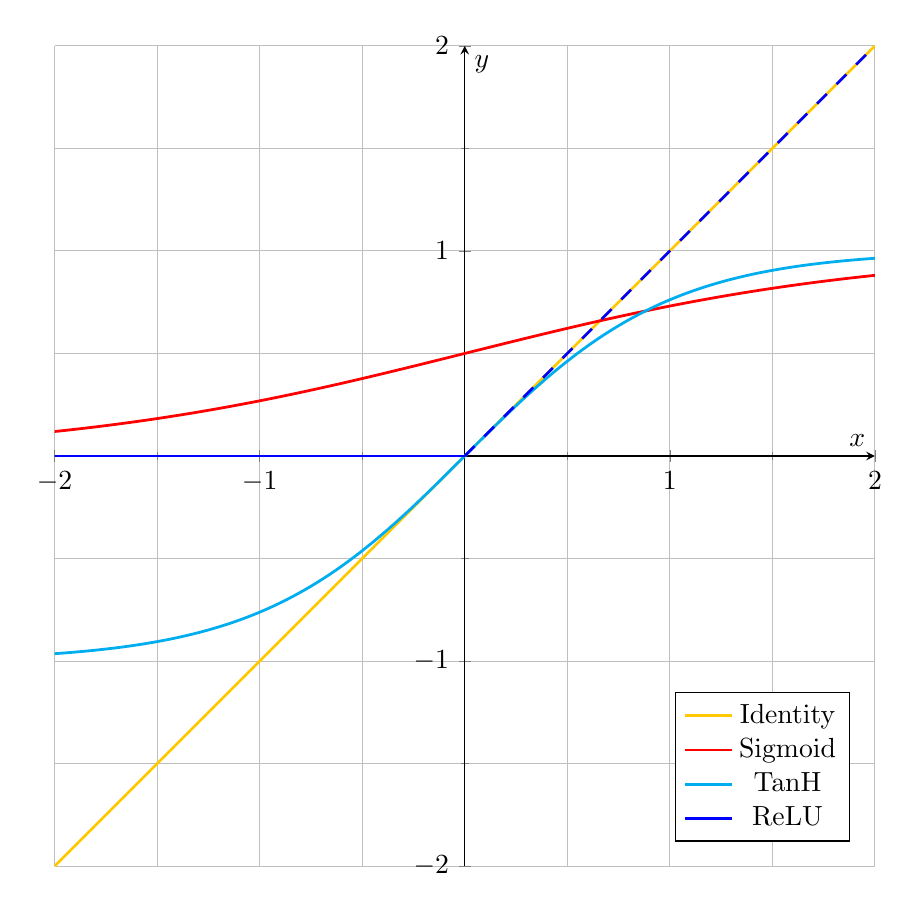
\begin{tikzpicture}
    \begin{axis}[width=12cm, height=12cm, axis lines=center, xtick={-2,...,2}, ytick={-2,...,2}, xmin=-2, xmax=2, ymin=-2, ymax=2, xlabel=$x$, ylabel=$y$, grid=both, minor tick num=1, legend pos=south east]
    
    \addplot[domain=-3:3, samples=500, line width=1, darkyellow] {x};
    \addlegendentry{Identity}
    
    \addplot[domain=-3:3, samples=500, line width=1, red] {1/(1+exp(-x))};
    \addlegendentry{Sigmoid}
    
    \addplot[domain=-3:3, samples=500, line width=1, cyan] {(exp(x) - exp(-x))/(exp(x) + exp(-x))};
    \addlegendentry{TanH}
    
    \addplot[domain=-3:0, samples=500, line width=1, blue] {0};
    \addplot[domain=0:3, samples=500, line width=1, dash pattern=on 5pt off 5pt, blue] {x};
    \addlegendentry{ReLU}
    
    \end{axis}
\end{tikzpicture}
\end{center}

\end{document}